
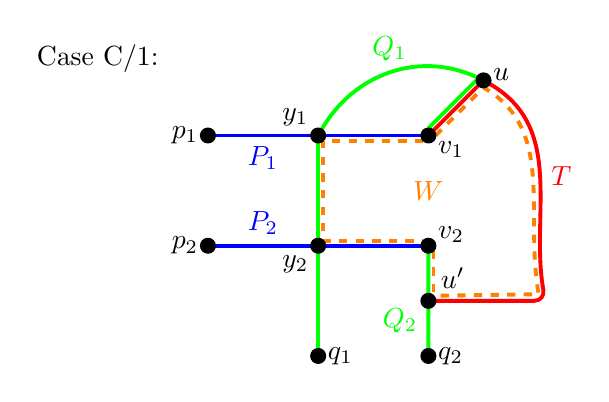
\begin{tikzpicture}[xscale=0.7, yscale=0.7]

  % vertices
  \node (C1) at (-4,3.4) {Case C/1:};
  \node[draw, circle, fill=black, inner sep=1.7pt] (y2) at (0, 0) {};
  \node[draw, circle, fill=black, inner sep=1.7pt] (y1) at (0, 2) {};  
  \node[draw, circle, fill=black, inner sep=1.7pt] (p2) at (-2, 0) {};
  \node[draw, circle, fill=black, inner sep=1.7pt] (p1) at (-2, 2) {};
  \node[draw, circle, fill=black, inner sep=1.7pt] (v2) at (2, 0) {};
  \node[draw, circle, fill=black, inner sep=1.7pt] (v1) at (2, 2) {};
  \node[draw, circle, fill=black, inner sep=1.7pt] (u) at (3, 3) {};
  \node[draw, circle, fill=black, inner sep=1.7pt] (q1) at (0, -2) {};
  \node[draw, circle, fill=black, inner sep=1.7pt] (q2) at (2, -2) {};
  \node[draw, circle, fill=black, inner sep=1.7pt] (u') at (2, -1) {};
  \coordinate (h) at (4, -0.88) {};
  \coordinate (h') at (4.12, -1) {};

  % names of vertices
  \node[left] at (p1) {$p_1$};
  \node[left] at (p2) {$p_2$};
  \node[above left] at (y1) {$y_1$};
  \node[below left] at (y2) {$y_2$};
  \node[right] at (q2) {$q_2$};  
  \node[right] at (q1) {$q_1$};    
  \node[right, yshift=-5pt] at (v1) {$v_1$};    
  \node[right, yshift=4pt] at (v2) {$v_2$};  
  \node[above right, yshift=1pt, xshift=1pt] at (u') {$u'$};    
  \node[right, yshift=2pt] at (u) {$u$};      
%  \node[right, xshift=-6pt, yshift=7pt] at (b.north) {$b$};

  % arcs
  \draw[line width=1.4pt, blue] (p1) to node[midway,below] {$P_1$} (y1);
  \draw[line width=1.4pt, blue] (y1) to (v1);  
  \draw[line width=1.4pt, blue] (p2) to node[midway,above] {$P_2$} (y2);  
  \draw[line width=1.4pt, blue] (y2) to (v2);
  \draw[line width=1.4pt, green] (v1.north) to (u.west);       
  \draw[line width=1.4pt, green] (q1) to (y2);    
  \draw[line width=1.4pt, green] (y2) to (y1);    
  \draw[line width=1.4pt, green] (q1) to (y2);    
  \draw[line width=1.4pt, green] (y2) to (y1);    
  \draw[line width=1.4pt, green] (y1) to[in=155, out=60] node[midway,above] {$Q_1$} (u);    
  \draw[line width=1.4pt, green] (v2) to (u');    
  \draw[line width=1.4pt, green] (u') to node[pos=0.3,left] {$Q_2$} (q2);      

  \draw[line width=1.4pt, red, rounded corners] (v1) to (u) to[out=-30, in=100] node[midway,right] {$T$} (h') to (u');

  
  \draw[line width=1.4pt, orange, dashed] (v1.east) to (u.south) to[out=-30, in=100] (h) to (u'.north east);    
  \draw[line width=1.4pt, orange, dashed] (v1.south west) to (y1.south east) to (y2.north  east) to (v2.north west);    
  \draw[line width=1.4pt, orange, dashed] (v2.south east) to (u'.north east);    
  
  \node[draw, circle, fill=black, inner sep=1.9pt] (y2) at (0, 0) {};
  \node[draw, circle, fill=black, inner sep=1.9pt] (y1) at (0, 2) {};  
  \node[draw, circle, fill=black, inner sep=1.9pt] (p2) at (-2, 0) {};
  \node[draw, circle, fill=black, inner sep=1.9pt] (p1) at (-2, 2) {};
  \node[draw, circle, fill=black, inner sep=1.9pt] (v2) at (2, 0) {};
  \node[draw, circle, fill=black, inner sep=1.9pt] (v1) at (2, 2) {};
  \node[draw, circle, fill=black, inner sep=1.9pt] (u) at (3, 3) {};
  \node[draw, circle, fill=black, inner sep=1.9pt] (q1) at (0, -2) {};
  \node[draw, circle, fill=black, inner sep=1.9pt] (q2) at (2, -2) {};
  \node[draw, circle, fill=black, inner sep=1.9pt] (u') at (2, -1) {};
  \node (W) at (2,1) [orange] {$W$};

\end{tikzpicture}


















